\appendixpageoff
\begin{appendices}




\chapter{Classification}
\section{Reults}
We detail the statistical values of the accuracy results of the trained models described in Section \ref{classificationEvaluation}.

\begin{table}[ht!]
\centering
\scalebox{0.95}{
\begin{tabular}{c|cccccc}
 \toprule
\rowcolor[HTML]{EEF9FB} 
{\color[HTML]{000000} \textbf{\begin{tabular}[c]{@{}c@{}}\rowcolor[HTML]{EEF9FB} Plot\\\rowcolor[HTML]{EEF9FB}  values\end{tabular}}} & {\color[HTML]{000000} \textbf{\begin{tabular}[c]{@{}c@{}}\rowcolor[HTML]{EEF9FB} Upper\\ \rowcolor[HTML]{EEF9FB} whisker\end{tabular}}} & {\color[HTML]{000000} \textbf{\begin{tabular}[c]{@{}c@{}}\rowcolor[HTML]{EEF9FB} 3rd \\ \rowcolor[HTML]{EEF9FB} quartile\end{tabular}}} & {\color[HTML]{000000} \textbf{Median}} & {\color[HTML]{000000} \textbf{\begin{tabular}[c]{@{}c@{}}\rowcolor[HTML]{EEF9FB} 1st \\ \rowcolor[HTML]{EEF9FB} quartile\end{tabular}}} & {\color[HTML]{000000} \textbf{\begin{tabular}[c]{@{}c@{}}\rowcolor[HTML]{EEF9FB} Lower\\ \rowcolor[HTML]{EEF9FB} whisker\end{tabular}}} & {\color[HTML]{000000} \textbf{Mean}} \\ 
 \midrule
\rowcolor[HTML]{DAE8E5} 
{\color[HTML]{000000} \textbf{C1}} & {\color[HTML]{000000} 0.00} & {\color[HTML]{000000} 0.00} & {\color[HTML]{000000} 0.00} & {\color[HTML]{000000} 0.00} & {\color[HTML]{000000} 0.00} & {\color[HTML]{000000} 0.00} \\
\rowcolor[HTML]{EEF9FB} 
{\color[HTML]{000000} \textbf{C2}} & {\color[HTML]{000000} 72.41} & {\color[HTML]{000000} 70.83} & {\color[HTML]{000000} 59.74} & {\color[HTML]{000000} 46.67} & {\color[HTML]{000000} 40.00} & {\color[HTML]{000000} 57.59} \\
\rowcolor[HTML]{DAE8E5} 
{\color[HTML]{000000} \textbf{C3}} & {\color[HTML]{000000} 100.00} & {\color[HTML]{000000} 76.92} & {\color[HTML]{000000} 70.84} & {\color[HTML]{000000} 58.33} & {\color[HTML]{000000} 10.00} & {\color[HTML]{000000} 66.43} \\
\rowcolor[HTML]{EEF9FB} 
{\color[HTML]{000000} \textbf{C4}} & {\color[HTML]{000000} 33.33} & {\color[HTML]{000000} 0.00} & {\color[HTML]{000000} 0.00} & {\color[HTML]{000000} 0.00} & {\color[HTML]{000000} 0.00} & {\color[HTML]{000000} 5.00} \\
\rowcolor[HTML]{DAE8E5} 
{\color[HTML]{000000} \textbf{C5}} & {\color[HTML]{000000} 91.67} & {\color[HTML]{000000} 61.54} & {\color[HTML]{000000} 51.92} & {\color[HTML]{000000} 33.33} & {\color[HTML]{000000} 22.22} & {\color[HTML]{000000} 50.66} \\
\rowcolor[HTML]{EEF9FB} 
{\color[HTML]{000000} \textbf{C6}} & {\color[HTML]{000000} 97.30} & {\color[HTML]{000000} 95.89} & {\color[HTML]{000000} 93.46} & {\color[HTML]{000000} 90.71} & {\color[HTML]{000000} 65.10} & {\color[HTML]{000000} 90.70} \\
\rowcolor[HTML]{DAE8E5} 
{\color[HTML]{000000} \textbf{C7}} & {\color[HTML]{000000} 100.00} & {\color[HTML]{000000} 66.67} & {\color[HTML]{000000} 58.34} & {\color[HTML]{000000} 20.00} & {\color[HTML]{000000} 0.00} & {\color[HTML]{000000} 49.00} \\
\rowcolor[HTML]{EEF9FB} 
{\color[HTML]{000000} \textbf{C8}} & {\color[HTML]{000000} 50.00} & {\color[HTML]{000000} 50.00} & {\color[HTML]{000000} 39.28} & {\color[HTML]{000000} 0.00} & {\color[HTML]{000000} 0.00} & {\color[HTML]{000000} 27.86} \\
\rowcolor[HTML]{DAE8E5} 
{\color[HTML]{000000} \textbf{C9}} & {\color[HTML]{000000} 88.76} & {\color[HTML]{000000} 83.75} & {\color[HTML]{000000} 78.33} & {\color[HTML]{000000} 73.49} & {\color[HTML]{000000} 53.01} & {\color[HTML]{000000} 75.52} \\
\rowcolor[HTML]{EEF9FB} 
{\color[HTML]{000000} \textbf{C10}} & {\color[HTML]{000000} 74.29} & {\color[HTML]{000000} 70.00} & {\color[HTML]{000000} 67.82} & {\color[HTML]{000000} 58.06} & {\color[HTML]{000000} 33.33} & {\color[HTML]{000000} 62.82} \\
\rowcolor[HTML]{DAE8E5} 
{\color[HTML]{000000} \textbf{C11}} & {\color[HTML]{000000} 92.26} & {\color[HTML]{000000} 90.73} & {\color[HTML]{000000} 88.54} & {\color[HTML]{000000} 85.21} & {\color[HTML]{000000} 80.00} & {\color[HTML]{000000} 87.84} \\
\rowcolor[HTML]{EEF9FB} 
{\color[HTML]{000000} \textbf{C12}} & {\color[HTML]{000000} 97.21} & {\color[HTML]{000000} 96.30} & {\color[HTML]{000000} 95.10} & {\color[HTML]{000000} 92.99} & {\color[HTML]{000000} 91.75} & {\color[HTML]{000000} 94.69} \\
\rowcolor[HTML]{DAE8E5} 
{\color[HTML]{000000} \textbf{C13}} & {\color[HTML]{000000} 47.06} & {\color[HTML]{000000} 34.78} & {\color[HTML]{000000} 34.05} & {\color[HTML]{000000} 30.43} & {\color[HTML]{000000} 21.05} & {\color[HTML]{000000} 33.58} \\
\rowcolor[HTML]{EEF9FB} 
{\color[HTML]{000000} \textbf{C14}} & {\color[HTML]{000000} 93.97} & {\color[HTML]{000000} 91.38} & {\color[HTML]{000000} 86.27} & {\color[HTML]{000000} 85.34} & {\color[HTML]{000000} 81.73} & {\color[HTML]{000000} 87.54} \\
\bottomrule
\end{tabular}
}
\caption{The statistical values of training on the first samples. The visualization is shown in Figure \ref{CM1Boxplot}.}
\label{CM1BoxplotValues}
\end{table}

\begin{table}[h]
\centering
\scalebox{0.95}{
\begin{tabular}{@{}c|cccccc@{}}
 \toprule
\rowcolor[HTML]{EEF9FB} 
{\color[HTML]{000000} \textbf{\begin{tabular}[c]{@{}c@{}}\rowcolor[HTML]{EEF9FB} Plot\\\rowcolor[HTML]{EEF9FB}  values\end{tabular}}} & {\color[HTML]{000000} \textbf{\begin{tabular}[c]{@{}c@{}}\rowcolor[HTML]{EEF9FB} Upper\\ \rowcolor[HTML]{EEF9FB} whisker\end{tabular}}} & {\color[HTML]{000000} \textbf{\begin{tabular}[c]{@{}c@{}}\rowcolor[HTML]{EEF9FB} 3rd \\ \rowcolor[HTML]{EEF9FB} quartile\end{tabular}}} & {\color[HTML]{000000} \textbf{Median}} & {\color[HTML]{000000} \textbf{\begin{tabular}[c]{@{}c@{}}\rowcolor[HTML]{EEF9FB} 1st \\ \rowcolor[HTML]{EEF9FB} quartile\end{tabular}}} & {\color[HTML]{000000} \textbf{\begin{tabular}[c]{@{}c@{}}\rowcolor[HTML]{EEF9FB} Lower\\ \rowcolor[HTML]{EEF9FB} whisker\end{tabular}}} & {\color[HTML]{000000} \textbf{Mean}} \\ 
\midrule
\rowcolor[HTML]{DAE8E5} 
\textbf{C2} & 97.31 & 94.97 & 94.47 & 93.20 & 90.40 & 94.09 \\
\rowcolor[HTML]{EEF9FB} 
\textbf{C6} & 96.60 & 95.97 & 92.59 & 91.45 & 68.57 & 91.00 \\
\rowcolor[HTML]{DAE8E5} 
\textbf{C7} & 98.08 & 97.87 & 97.47 & 91.67 & 89.58 & 95.12 \\
\rowcolor[HTML]{EEF9FB} 
\textbf{C9} & 98.80 & 89.74 & 82.57 & 78.31 & 71.05 & 84.07 \\
\rowcolor[HTML]{DAE8E5} 
\textbf{C15} & 86.84 & 66.67 & 63.82 & 43.33 & 30.56 & 60.13 \\
\rowcolor[HTML]{EEF9FB} 
\textbf{C10} & 76.67 & 71.43 & 65.97 & 52.94 & 45.16 & 63.08 \\
\rowcolor[HTML]{DAE8E5} 
\textbf{C11} & 94.34 & 90.00 & 86.94 & 82.24 & 54.04 & 84.00 \\
\rowcolor[HTML]{EEF9FB} 
\textbf{C12} & 69.81 & 68.18 & 66.37 & 60.71 & 57.14 & 64.72 \\
\rowcolor[HTML]{DAE8E5} 
\textbf{C13} & 65.22 & 42.86 & 29.48 & 17.24 & 2.86 & 30.29 \\
\rowcolor[HTML]{EEF9FB} 
\textbf{C14} & 95.33 & 89.08 & 87.77 & 84.82 & 80.19 & 87.63 \\
\bottomrule
\end{tabular}
}
\caption{The statistical values of training on the enhanced samples.  The visualization is portrayed in Figure \ref{CM2Boxplot}.}
\label{CM2BoxplotValues}
\end{table}

\begin{table}[]
\centering
\scalebox{0.95}{
\begin{tabular}{@{}c|cccccc@{}}
 \toprule
\rowcolor[HTML]{EEF9FB} 
{\color[HTML]{000000} \textbf{\begin{tabular}[c]{@{}c@{}}\rowcolor[HTML]{EEF9FB} Plot\\\rowcolor[HTML]{EEF9FB}  values\end{tabular}}} & {\color[HTML]{000000} \textbf{\begin{tabular}[c]{@{}c@{}}\rowcolor[HTML]{EEF9FB} Upper\\ \rowcolor[HTML]{EEF9FB} whisker\end{tabular}}} & {\color[HTML]{000000} \textbf{\begin{tabular}[c]{@{}c@{}}\rowcolor[HTML]{EEF9FB} 3rd \\ \rowcolor[HTML]{EEF9FB} quartile\end{tabular}}} & {\color[HTML]{000000} \textbf{Median}} & {\color[HTML]{000000} \textbf{\begin{tabular}[c]{@{}c@{}}\rowcolor[HTML]{EEF9FB} 1st \\ \rowcolor[HTML]{EEF9FB} quartile\end{tabular}}} & {\color[HTML]{000000} \textbf{\begin{tabular}[c]{@{}c@{}}\rowcolor[HTML]{EEF9FB} Lower\\ \rowcolor[HTML]{EEF9FB} whisker\end{tabular}}} & {\color[HTML]{000000} \textbf{Mean}} \\ 
\midrule
\rowcolor[HTML]{DAE8E5} 
\textbf{C6} & 95.77 & 94.66 & 90.47 & 90.00 & 86.92 & 91.38 \\
\rowcolor[HTML]{EEF9FB} 
\textbf{C7} & 100.00 & 96.00 & 95.29 & 92.68 & 75.56 & 93.26 \\
\rowcolor[HTML]{DAE8E5} 
\textbf{C8} & 92.86 & 80.68 & 73.37 & 64.04 & 46.67 & 72.02 \\
\rowcolor[HTML]{EEF9FB} 
\textbf{C9} & 88.89 & 84.21 & 75.12 & 65.38 & 46.43 & 73.05 \\
\rowcolor[HTML]{DAE8E5} 
\textbf{C10} & 77.27 & 70.97 & 68.20 & 65.00 & 58.82 & 68.18 \\
\rowcolor[HTML]{EEF9FB} 
\textbf{C11} & 92.31 & 88.03 & 86.18 & 85.44 & 78.12 & 86.19 \\
\rowcolor[HTML]{DAE8E5} 
\textbf{C16} & 98.36 & 96.86 & 96.63 & 95.80 & 94.44 & 96.50 \\
\rowcolor[HTML]{EEF9FB} 
\textbf{C13} & 62.07 & 40.74 & 35.71 & 30.00 & 13.79 & 36.49 \\
\rowcolor[HTML]{DAE8E5} 
\textbf{C14} & 94.12 & 92.44 & 88.69 & 84.96 & 83.61 & 88.63 \\
\bottomrule
\end{tabular}
}
\caption{The statistical accuracy values of training on the final samples. The portrayal is depicted in Figure \ref{CM3Boxplot}.}
\label{CM3BoxplotValues}
\end{table}

\begin{table}[]
\centering
\scalebox{0.95}{
\begin{tabular}{@{}c|cccccc@{}}
 \toprule
\rowcolor[HTML]{EEF9FB} 
{\color[HTML]{000000} \textbf{\begin{tabular}[c]{@{}c@{}}\rowcolor[HTML]{EEF9FB} Plot\\\rowcolor[HTML]{EEF9FB}  values\end{tabular}}} & {\color[HTML]{000000} \textbf{\begin{tabular}[c]{@{}c@{}}\rowcolor[HTML]{EEF9FB} Upper\\ \rowcolor[HTML]{EEF9FB} whisker\end{tabular}}} & {\color[HTML]{000000} \textbf{\begin{tabular}[c]{@{}c@{}}\rowcolor[HTML]{EEF9FB} 3rd \\ \rowcolor[HTML]{EEF9FB} quartile\end{tabular}}} & {\color[HTML]{000000} \textbf{Median}} & {\color[HTML]{000000} \textbf{\begin{tabular}[c]{@{}c@{}}\rowcolor[HTML]{EEF9FB} 1st \\ \rowcolor[HTML]{EEF9FB} quartile\end{tabular}}} & {\color[HTML]{000000} \textbf{\begin{tabular}[c]{@{}c@{}}\rowcolor[HTML]{EEF9FB} Lower\\ \rowcolor[HTML]{EEF9FB} whisker\end{tabular}}} & {\color[HTML]{000000} \textbf{Mean}} \\ 
\midrule
\rowcolor[HTML]{DAE8E5} 
\textbf{C6} & 97.97 & 96.00 & 94.13 & 92.09 & 86.15 & 93.70 \\
\rowcolor[HTML]{EEF9FB} 
\textbf{C7} & 98.15 & 97.44 & 96.11 & 94.87 & 90.48 & 95.72 \\
\rowcolor[HTML]{DAE8E5} 
\textbf{C8} & 98.63 & 85.71 & 75.45 & 57.97 & 42.31 & 72.44 \\
\rowcolor[HTML]{EEF9FB} 
\textbf{C9} & 88.89 & 83.33 & 64.87 & 50.00 & 8.33 & 60.95 \\
\rowcolor[HTML]{DAE8E5} 
\textbf{C10} & 82.35 & 75.00 & 66.89 & 58.62 & 32.00 & 64.49 \\
\rowcolor[HTML]{EEF9FB} 
\textbf{C11} & 90.45 & 88.16 & 86.01 & 81.37 & 27.11 & 80.02 \\
\rowcolor[HTML]{DAE8E5} 
\textbf{C16} & 98.71 & 97.24 & 96.74 & 96.54 & 92.53 & 96.36 \\
\rowcolor[HTML]{EEF9FB} 
\textbf{C13} & 68.42 & 58.06 & 45.86 & 37.04 & 0.00 & 44.17 \\
\rowcolor[HTML]{DAE8E5} 
\textbf{C14} & 93.75 & 89.86 & 86.76 & 84.68 & 75.86 & 86.74 \\
\bottomrule
\end{tabular}
}
\caption{The statistical accuracy values of training on the final samples with pretrained embeddings. The visualization is shown in Figure \ref{CM3EmbeddingsBoxplot}.}
\label{CM3EmbeddingsBoxplotValues}
\end{table}

\begin{table}[]
\centering
\scalebox{0.83}{
\begin{tabular}{@{}c|cccccc@{}}
 \toprule
\rowcolor[HTML]{EEF9FB} 
{\color[HTML]{000000} \textbf{\begin{tabular}[c]{@{}c@{}}\rowcolor[HTML]{EEF9FB} Plot\\\rowcolor[HTML]{EEF9FB}  values\end{tabular}}} & {\color[HTML]{000000} \textbf{\begin{tabular}[c]{@{}c@{}}\rowcolor[HTML]{EEF9FB} Upper\\ \rowcolor[HTML]{EEF9FB} whisker\end{tabular}}} & {\color[HTML]{000000} \textbf{\begin{tabular}[c]{@{}c@{}}\rowcolor[HTML]{EEF9FB} 3rd \\ \rowcolor[HTML]{EEF9FB} quartile\end{tabular}}} & {\color[HTML]{000000} \textbf{Median}} & {\color[HTML]{000000} \textbf{\begin{tabular}[c]{@{}c@{}}\rowcolor[HTML]{EEF9FB} 1st \\ \rowcolor[HTML]{EEF9FB} quartile\end{tabular}}} & {\color[HTML]{000000} \textbf{\begin{tabular}[c]{@{}c@{}}\rowcolor[HTML]{EEF9FB} Lower\\ \rowcolor[HTML]{EEF9FB} whisker\end{tabular}}} & {\color[HTML]{000000} \textbf{Mean}} \\ 
\midrule
\rowcolor[HTML]{DAE8E5} 
\textbf{first samples} & 86.11 & 85.38 & 84.77 & 82.22 & 76.98 & 83.65 \\
\rowcolor[HTML]{EEF9FB} 
\textbf{enhanced samples} & 86.69 & 85.76 & 85.01 & 81.25 & 77.78 & 83.81 \\
\rowcolor[HTML]{DAE8E5} 
\textbf{final samples} & 88.19 & 87.73 & 86.86 & 85.88 & 81.37 & 86.41 \\
\rowcolor[HTML]{EEF9FB} 
\textbf{final samples E} & 89.24 & 88.54 & 86.11 & 84.95 & 72.69 & 85.41 \\
\bottomrule
\end{tabular}
}
\caption{The statistical values of the overall accuracy of training on individual data sets. This is depicted in Figure \ref{DSsBoxplot}.}
\label{DSsBoxplotValues}
\end{table}





\chapter{Clustering comparison} \label{dixClustering}
\section{Number of communities comparison} \label{dixNumberOfCommunitiesComparison}
\begin{figure}[ht!]
  \centering
  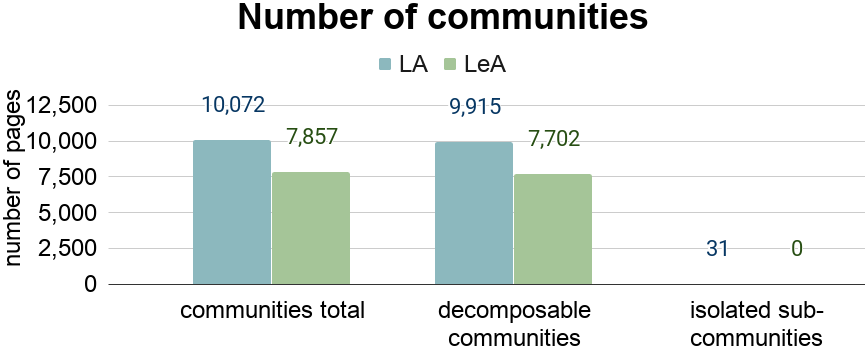
\includegraphics[width=\textwidth]{Images/CommunitiesComparison.png}
  \caption{The number of communities detected by the LA and LeA compared. }
  \label{CommunitiesComparison}
\end{figure}

\section{Partition execution times comparison} \label{dixExecutionTimesComparison}
\begin{figure}[ht!]
  \centering
  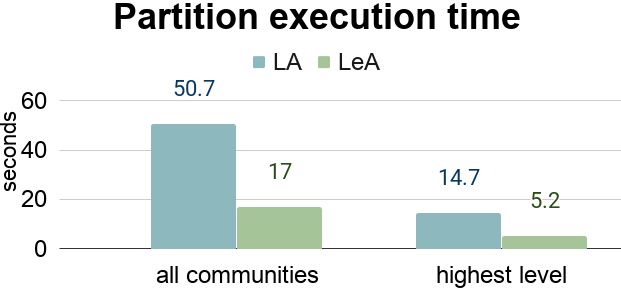
\includegraphics[width=0.8\textwidth]{Images/PartitionTimeComparison.png}
  \caption{The amount of time it took the LA amd LeA to detect communities compared.}
  \label{PartitionTimeComparison}
\end{figure}







\chapter{Imeplementation details}
\section{Classification}
\subsection{Embedding vector} \label{dix_embeddingVector}
We enclose a portion of an embedding vector for the words \textit{email} copied from the embedding index of the embedding layer.

\texttt{array([\\
 -0.57792, -0.16606, -0.17226, -0.87941,  0.30588,\\
...,\\
  0.052887, 0.077703, -0.10182, -0.33831, 0.55555\\
], dtype=float32)}

\subsection{Vocabulary initialization}
\subsection{Data set vocabulary} \label{DSvocabulary}
We enclose a portion of the vocabulary created from our data set.

\texttt{
\{\\
\text{    }"1": "porn", "2": "porno", "3": "the", "4": "to", ...,\\
    ...,\\
    ..., "129988": "3e3zx2drxj", "129989":"tapasoth"\\
\}}

\section{API}
\subsection{Classification} \label{dixApClassification}
The class Categorizer first loads the tokenizer and the trained model. Then the model is compiled with the same attributes as described in Subsection \ref{ClassificationImplementation}. Both the tokenizer and the model are utilized in the method \texttt{categorize}. This method expects the page content as parameter. It applies the tokenizer to the received content. The output is padded or concatenated to the same length of 1,000 digits. The model predicts the category alias of the modified content. Lastly, the alias is converted to the name of the category.
\FloatBarrier 
\subsection{Models} \label{dixModels}
\begin{figure}[ht!]
  \centering
  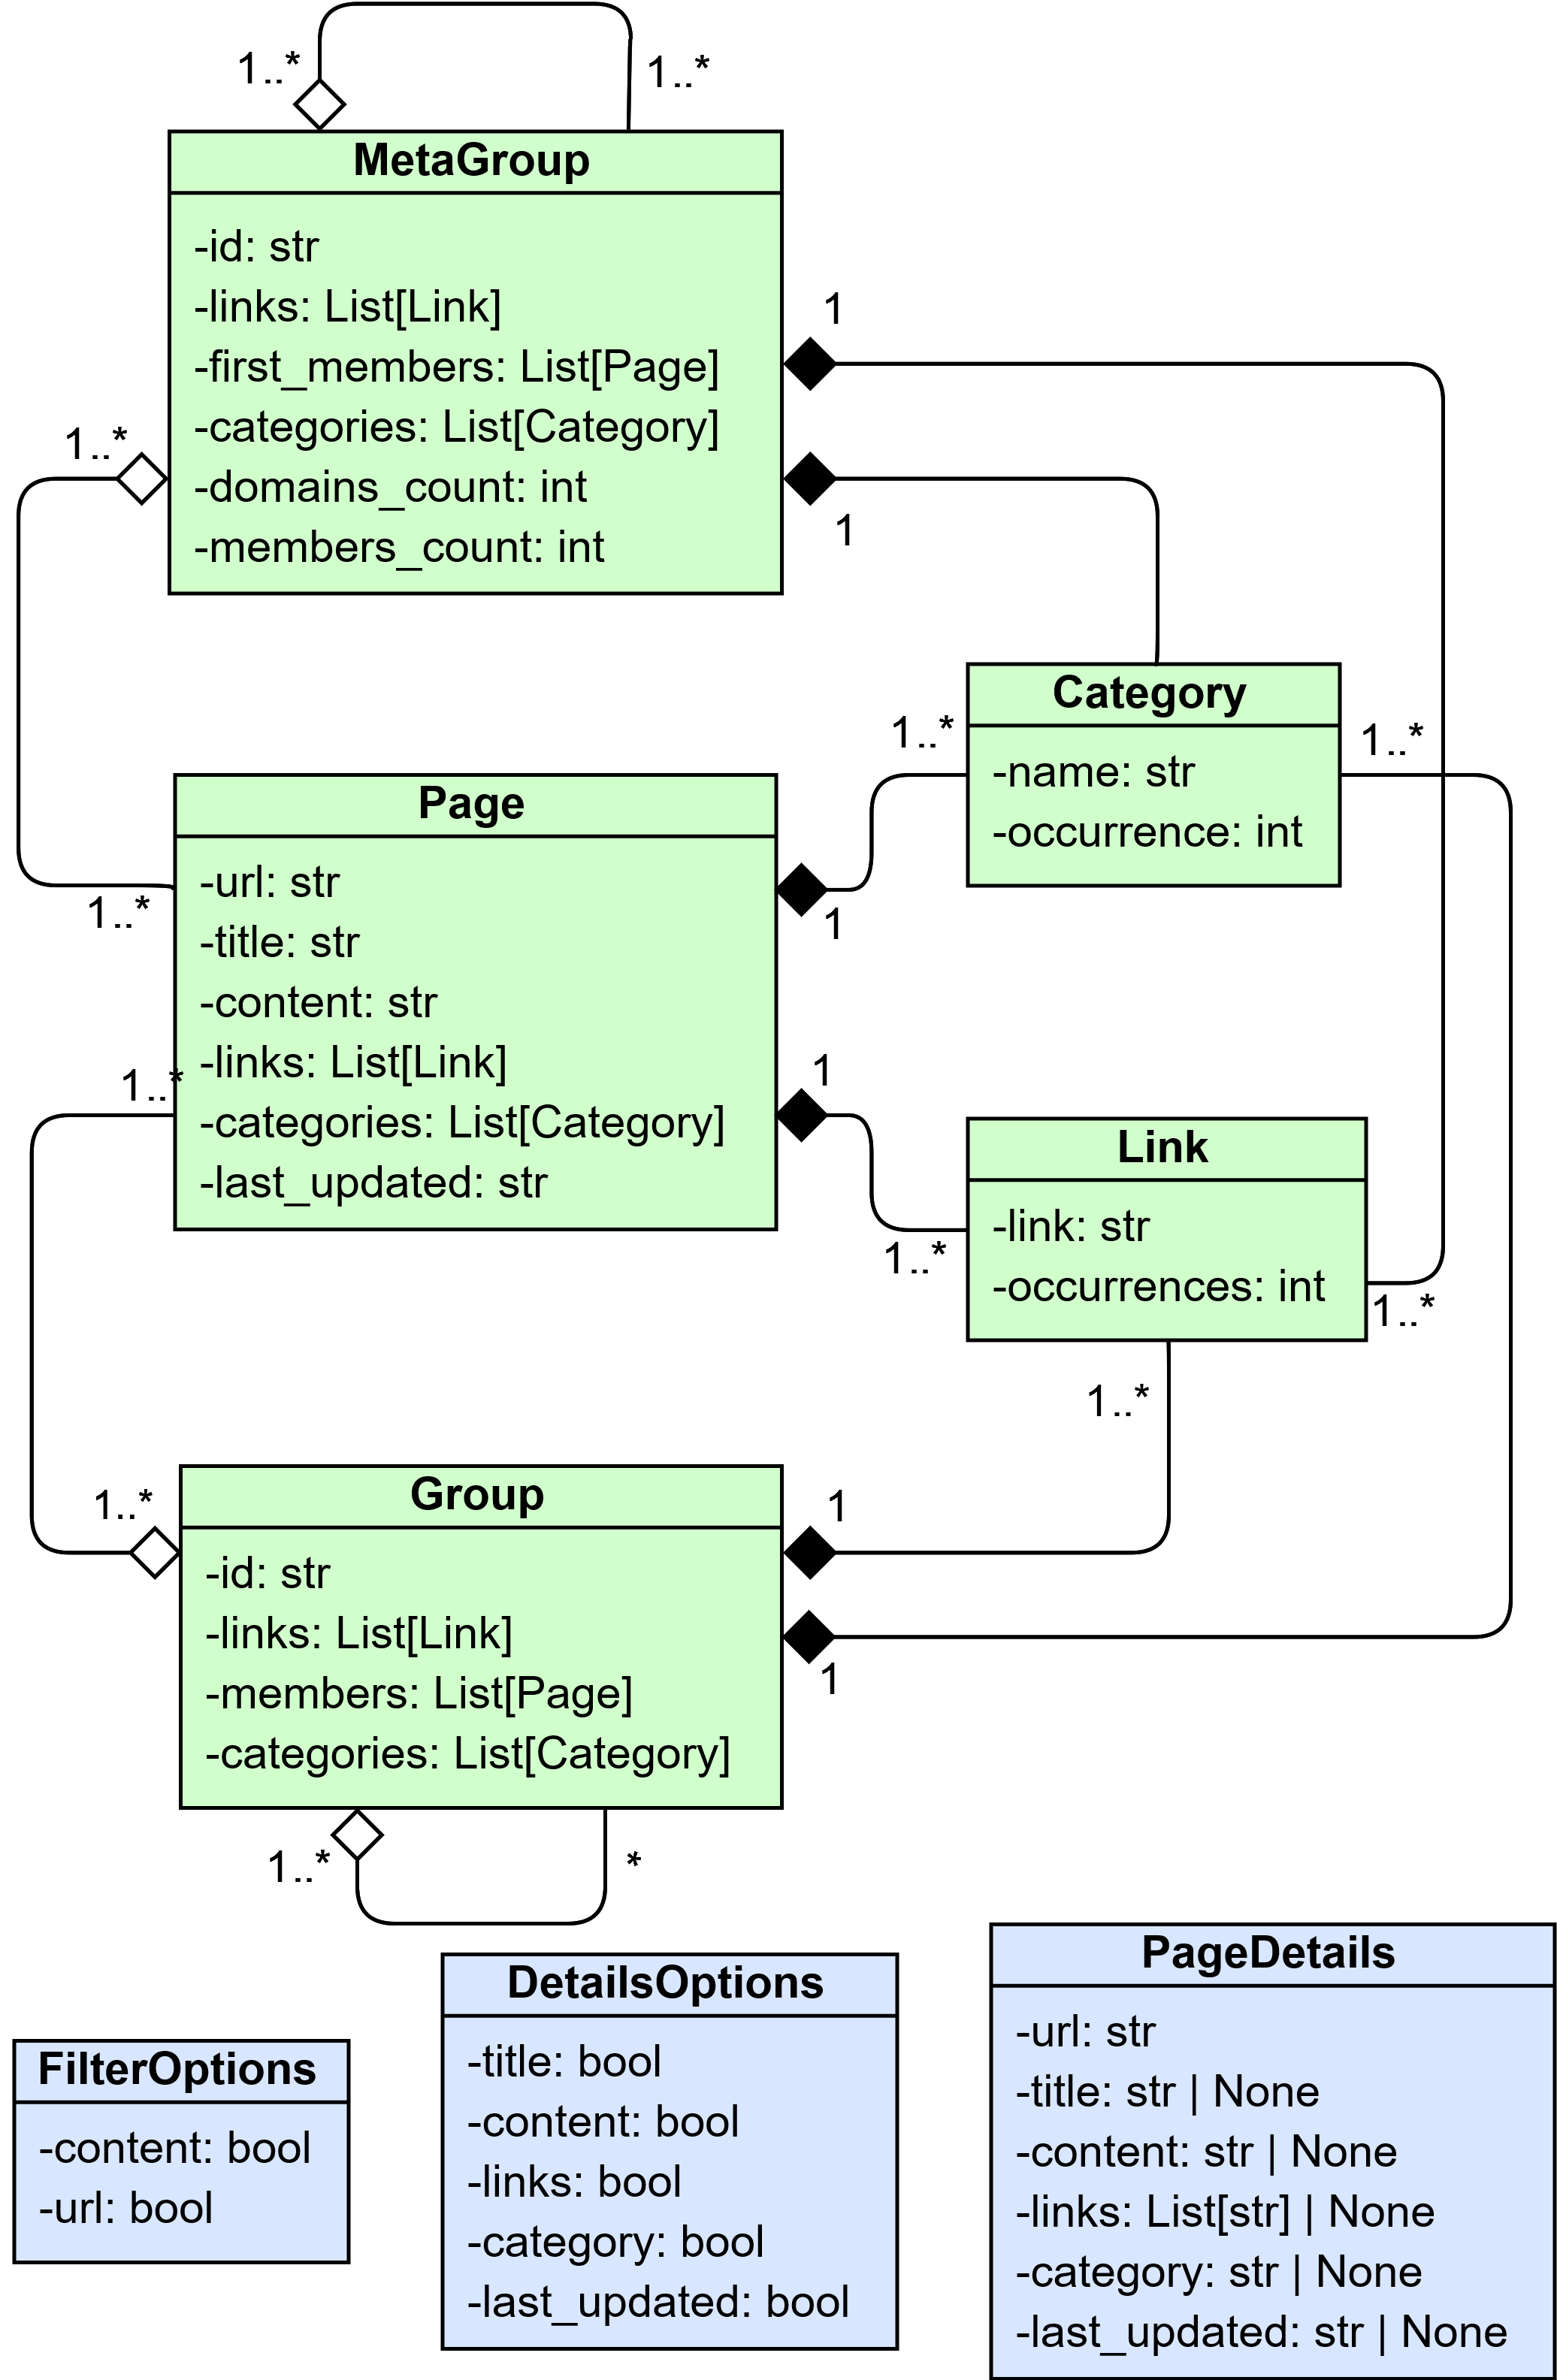
\includegraphics[height=0.85\textheight]{Images/BEmodelsDiagram.png}
  \caption{A class diagram of the classes used in the BE. The diagram was created leveraging Visual Paradigm \cite{visualParadigm}}
  \label{BEmodelsDiagram}
\end{figure}
\FloatBarrier 
\subsection{Response example} \label{dixAPIResponse}
 We now detail an example of handeling a response. The API structure is described in Subsection \ref{APIImplementation}. Let us assume the API received the request 
\begin{quotation}
 \texttt{GET /api/pages/bylink/?content-type=json\&id=2.0} . 
\end{quotation}
The client now expects the API to return sub-communities of the community with the id \textit{2.0}. The ViewSet \texttt{GroupsByLinkViewSet} is assigned to the used endpoint. The method used in the request is \textit{GET}. Therefore the \textit{list} function of \texttt{GroupsByLinkViewSet} is called. The url provided contains the \texttt{id} parameter. The helper method \\ \texttt{get\_subgroups\_of\_group} with the provided \texttt{id} is called. 

The method caches and returns a list of \texttt{Group} objects. However, this response would be too sizable for the server-client communication. That is why the \texttt{Group} objects are converted to \texttt{Meta\_Group} objects. A \texttt{Meta\_Group} object doe not contain all of the community pages. It contains only the first 10 pages as \texttt{Page} objects. \texttt{Meta\_Group} also contains an attribute representing the number of the pages. The list of \texttt{Meta\_Group} objects is serialized via the \texttt{MetaGroupSerializer}. 

At last a \texttt{Response} object is constructed with the serialized result as its data. The response is returned to the client.

\subsection{Page acquisition} \label{dixRepositories}
We detail the implementation of the different page acquisition methods.

Method \texttt{basic\_search} is used for the filtering of nodes based on page-content or page-ulr. 

Method \texttt{fetch\_chunk} retrieves portions with pages called \textit{chunks} from the database. In this thesis a chunk contains 500 pages. Each response from the database holds a chunk and a \textit{scroll\_id}. This id is sent in the next request to the database. The enclosed chunk in the next response from \textit{Elasticsearch}  depends on the scroll\_id. The search context of \textit{Elasticsearch} is kept open for 1 minute. This is defined by \texttt{scroll} attribute. Each request extends this time by another minute. 

Method \texttt{fetch\_all} gets all pages from the database. In this method \texttt{fetch\_chunk} is called repeatedly until the response carries no pages. Each chunk is converted to a dictionary of \texttt{Page} objects with the page url as key and the whole page as value. Also, each batch is stored on the disc in a \textit{shelf}. The keys in the \textit{shelf} are indexes of the batches and the values are the whole batches. After all pages from the database are obtained the content is removed from the pages. Also, invalid links are deleted from the pages. Then the pages are cached in \textit{Redis}.

\section{FE}
\subsection{Detailed file structure}
\begin{description}
    \item[\texttt{node\_modules}] contains imported libraries including \textit{React.js}, \textit{Redux} or \textit{d3}.
    \item[\texttt{public}] encloses a \textit{.ico} file\footnote {A picture with the dimensions 16x16 pixels used by the browser to represent the web page or application. It is usually displayed in the tab in which the application is opened.} and a html file which is the default entry point when the application is started. 
    \item[\texttt{}]
    \item[\texttt{}]
    \item[\texttt{}]
\end{description}
The folder \texttt{node\_modules} contains imported libraries including \textit{React.js}, \textit{Redux} or \textit{d3}. The next folder named \texttt{public} encloses a \textit{.ico} file\footnote {A picture with the dimensions 16x16 pixels used by the browser to represent the web page or application. It is usually displayed in the tab in which the application is opened.} and a html file which is the default entry point when the application is started. The last folder \texttt{src} contains the source code itself. 

As previously mentioned, the FE is written in \textit{TS} which has the advantage of readability and easy navigation. There are, however, also disadvantages. One of them is the need of a \textit{TS} file with the types (typing) for every used library. Typings for popular libraries are often downloadable as modules. If a library has no ready-to-download typings own ones need to be written. In our case the typings for the library \textit{react-d3-graph} were custom made. They can be found in the folder \texttt{@types/react-d3-graph}. The file \texttt{commont.d.ts} holds types used heavily across the application, e.g. \textit{Action}. Types in this file are available without importing them to all files in the project.

\subsection{Detailed fetchNode AC}\label{dixComplicatedAC}
The AC \texttt{fetchNodes} and the folder it is placed in share the same name. For easier testing purposes the main logic of this AC is put into a function which receives the simple ACs as dependencies. When this AC is called it first dispatches a simple AC to indicate the fetching has begun. After that an identificator (id) is initialized. This id is later used to create an error object in case of failure. Next, the fetching itself begins. The fetching in \texttt{fetchNodes} is realized with the library \textit{isomorphic-fetch}. The fetch function of this library expects the first argument to be the url address of the resource. The second argument is an object describing further details of the request and is optional. Such an object may contain the request method, headers or the payload. If the request does not result in error the response status is checked. After the fetching is complete a success AC with the acquired response is dispatched. If an error is caught during the fetching a failure AC is dispatched. The payload of this AC is an error-object with the id and error message if any.




\chapter{How to train a data set}
\chapter{How to start the the dark web visualization app}
\end{appendices}